\documentclass[]{aiaa-tc}% insert '[draft]' option to show overfull boxes

\usepackage[toc,page]{appendix} 
 \usepackage{varioref}%  smart page, figure, table, and equation referencing
 \usepackage{wrapfig}%   wrap figures/tables in text (i.e., Di Vinci style)
 \usepackage{threeparttable}% tables with footnotes
 \usepackage{dcolumn}%   decimal-aligned tabular math columns
  \newcolumntype{d}{D{.}{.}{-1}}
 \usepackage{nomencl}%   nomenclature generation via makeindex
  \makeglossary
 \usepackage{subfigure}% subcaptions for subfigures
 \usepackage{subfigmat}% matrices of similar subfigures, aka small mulitples
 \usepackage{fancyvrb}%  extended verbatim environments
  \fvset{fontsize=\footnotesize,xleftmargin=2em}
 \usepackage{lettrine}%  dropped capital letter at beginning of paragraph
% \usepackage[dvips]{dropping}% alternative dropped capital package
% \usepackage[colorlinks]{hyperref}%  hyperlinks [must be loaded after dropping]
%\usepackage{makeidx}


\graphicspath{{Images/}}
%\usepackage[colorlinks]{hyperref}
%\hypersetup{colorlinks = false}
\usepackage{url}

\usepackage{pdfpages}
\usepackage[ampersand]{easylist}

\usepackage{natbib}
\bibliographystyle{abbrvnat}
\setcitestyle{authoryear,open={(},close={)}}

%AJL SEIT Comment out these two lines for the final submission
%\usepackage{draftwatermark}
%\SetWatermarkFontSize{5cm} \SetWatermarkScale{6} \SetWatermarkText{\textbf{DRAFT-REMOVE}}
\pagestyle{plain}

 \title{Towards self driving: Single camera navigation localisation\\ Interim report}

 \author{
  Michael McDonnell\thanks{CAPT, School of Engineering and Information Technology, ZEIT4901}\
  \\
  {\normalsize\itshape
   UNSW Canberra at ADFA.}\\
  }

 % Data used by 'handcarry' option
 %\AIAApapernumber{YEAR-NUMBER}
 %\AIAAconference{Conference Name, Date, and Location}
 %\AIAAcopyright{\AIAAcopyrightD{YEAR}}

 % Define commands to assure consistent treatment throughout document
% \newcommand{\eqnref}[1]{(\ref{#1})}
% \newcommand{\class}[1]{\texttt{#1}}
% \newcommand{\package}[1]{\texttt{#1}}
% \newcommand{\file}[1]{\texttt{#1}}
% \newcommand{\BibTeX}{\textsc{Bib}\TeX}

%\makeindex

\begin{document}

\maketitle


\begin{abstract}
The aim of this project is to investigate localising navigation data from a GPS feed to the observed road via a vehicle mounted camera. A subordinate aim as part of this is to develop a simulation that will provide sensor data to an external program for processing. A general motivation for this project is the development of a `low tech' solution which will enable automation of simple road movements, for example routine (non-tactical )military logistic resupply. 
The early focus for this project was developing core competencies in Image Processing and Computer Vision techniques which feed in to the design of the localisation system architecture. OpenCV in Python is used for the sensor analysis which includes GPS position data, navigation route information and video feed from a simulated vehicle.
The simulation design and tool analysis was conducted with the key technical risks addressed. The simulation is being developed in Unity and requires inter process communication between the Unity process and the external Python process. This has been developed using the ZeroMQ library and the simulation uses dynamic time scaling to ensure that sensor data processing occurs at a desired rate. The simulation development has now entered an agile design approach with iterative functionality improvements to be delivered.
The navigation localisation problem has key technical risks in curved lane and intersection detection and correlation of the detected features with the navigation data. Several candidate approaches to address these risks have been identified and work in these areas will be progressing in the short term with the likely candidates being intersection model based matching with road edge pixels.
\end{abstract}

\newpage
\tableofcontents

\newpage
\section{Introduction} \label{sect:intro}
%\index{}
 
\lettrine[nindent=0pt]{T}{he} idea of a future where personal transportation is handled by autonomous vehicles is increasingly in the public consciousness however there is a range of challenges that need to be addressed from legal, security and ethical issues \citep{gmReport} to maturity concerns that out to the 2030s, `autonomous vehicles will be expensive novelties' \citep{vicTransportImplications}. Autonomous driving is not a binary capability however, rather a scale with increasing levels of autonomy. For context, the automation levels identified by the US National Highway Traffic Safety Administration \citep{automationVisionForSafety} are outlined in table \ref{t:automationLevels}. While it may be decades before true level 5 automation is developed, there is an undeniable increase in the cognitive assistance and partial automation technologies in consumer vehicles. As an example the 2019 Kia Sorento includes active lane keeping assist (lane detection and steering) and adaptive cruise control (autonomous acceleration and braking based off radar distance to leading vehicles) \citep{kia}, aligning to level 2 automation. 


\begin{table}
 \begin{center}
  \caption{automation levels identified by the US National Highway Traffic Safety Administration \citep{automationVisionForSafety}}
  \label{t:automationLevels}
  \begin{tabular}{p{0.1\linewidth}p{0.25\linewidth}p{0.6\linewidth}}
       Level & Classification & Detail\\\hline
        0 &  No Automation & Zero autonomy; the driver performs all driving tasks. \\
       1 &  Driver Assistance & Vehicle is controlled by the driver, but some driving assist features may be included in the vehicle design \\
       2 &  Partial Automation & Vehicle has combined automated functions, like acceleration and steering, but the driver must remain engaged with the driving task and monitor the environment at all times. \\
       3 &  Conditional Automation &   Driver is a necessity, but is not required to monitor the environment. The driver must be ready to take control of the vehicle at all times with notice. \\
      4 &  High Automation &   The vehicle is capable of performing all driving functions under certain conditions. The driver may have the option to control the vehicle. \\
      5 &   Full Automation &   The vehicle is capable of performing all driving functions under all conditions. The driver may have the option to control the vehicle. 
  \end{tabular}
 \end{center}
\end{table}

In order for an autonomous vehicle to navigate effectively there are a few key challenges. The vehicle must have a mechanism to sense the local environment, for example lane detection, as well as the ability to identify and track transient aspects such as other vehicles and on road obstacles. There are many Computer Vision techniques that can assist in providing an understanding of the environment. Direct techniques such as edge and line detection are widely used however Deep Convolutional Neural Networks have also been shown to be effective for road detection \citep{deepRoadSegmentation}.

In addition to the local area, the vehicle must also have the ability to reconcile navigation data with the current location. A supporting concept to this is that of map matching which calculates vehicle location by using the geographical information from sensors such as GPS position and inertial data and the map information from the mapping service \citep{keyTechSelfDriving}. Current cutting edge self driving vehicles require high fidelity 3D maps to operate effectively which are time consuming to develop and not adaptive to rapid local changes. Despite this, position localisation improvements have been achieved without high fidelity 3D mapping data using a data fusion of GPS and inertial navigation system data \citep{gpsInsFusion} correlating a back lane mark registry supported with computer vision, GPS and inertial data with map data \citep{lowCostSensorNav} and through use of Kalman filters and LIDAR in more complex environments \citep{robotLIDARSLAM}.

This process of combining data from several sources into a single unified description of a situation is known as data fusion \citep{gpsInsFusion}. Self driving vehicles rely on sensor and data fusion to achieve the four capabilities required of autonomous driving; navigation, path planning, environment perception and car control \citep{keyTechSelfDriving}. This project touches on elements of the first three capabilities in order to localise navigation information. This project will use GPS position data and computer vision techniques to correlate data from preloaded maps to localise localise navigation. The context for this project is general but will loosely use the goal of automating (non-tactical) military field logistics route transport. This will include simplifying assumptions of single lane roads/tracks without the requirement to consider other vehicles or traffic control. The idea of local navigation goals has been explored with the use of Open Street Map data and LIDAR for road mapping with promising success \citep{mitLocalNavDriving} however the ability for a single camera system to facilitate navigation data localisation assists in both system redundancy and lowering the financial and technical barriers to implementation. This project will focus on a `low tech' option to provide a minimum navigation capability that does not rely on more advanced tools such as LIDAR. Consideration of comparable work will be further outlined in specific sections of current and future work as it is relevant.

In general, the ability to use computer vision to align GPS positioning with mapping service data will allow greater cognitive assistance in driver included tasks without the requirement for significant prior mapping. As augmented reality technology increases this also allows for more immersive driver aides such as navigation routes overlayed onto the visible road. In addition to the cognitive assistance, the ability to localise a navigation route opens the near future possibility for the automation of certain tasks in a military setting, for example routine field logistics supply transport. A true complete solution will rely on sensor fusion from a suit of complimentary sensors supporting each other and providing redundancy. 

\subsection{Terminology}

The following abbreviations and definitions are used throughout this report:

\begin{easylist}[itemize]
	& \textbf{Computer Vision (CV)}. Techniques to allow machines to `see'; processing visual images of the world and deriving understanding.
	& \textbf{Digital Image Processing (DIP)}. Use of computer algorithms to perform processing on digital images.
	& \textbf{Navigation localisation}. Translating an overall navigation route into a local navigation goal.
	& \textbf{Simulation}. The custom built autonomous vehicle simulation which provides sensor feed outputs.
	& \textbf{External processing}. In the context of this report two programs are discussed, the simulation and `external processing'. External processing refers to the standalone code which performs the computational calculations for navigation localisation.
	& \textbf{Simulation tick}. One period of simluation processing. This is aligned to a specified update frequency that the external processing is running at `in simulation'.
	& \textbf{Interprocess Communication (IPC)}. The passage of data from simulation to external processes.
	& \textbf{Open Street Maps (OSM)}. `A collaborative project to create a free editable map of the world' \citep{osmDataFormat}. Comparable to Google maps.
	& \textbf{Polyline}. A line defined by node coordinates. The line is drawn through all nodes in order, starting at the first and terminating at the last.
\end{easylist}

\subsection{Project aim}

The aim of this project is to investigate localising navigation data from a GPS feed to the observed road via a vehicle mounted camera. Mapping service GPS route data is often held as polylines which represents a road as a series of connected points or nodes \citep{googleMapPolyline}, \citep{osmDataFormat}. The approach for positional localisation is to use the vehicle GPS position as an approximate input location mapped to the closest point on a route. Detected road features are then used to determine an accurate position of the vehicle and identify the navigation route on forward facing video feed. This sets the conditions for autonomous control of the vehicle based on a programmed navigation route. 


A subordinate aim to the project is the development of a simulation which provides a sensor data, such as GPS location and video feeds from a simulated vehicle in 3D space. This simulation will allow both the generation of a large and varied data set for testing as well as allow the ability to provide control feedback for the simulated vehicle based on results from processing of the sensor data.

The data flow is anticipated to be as visualised in figure \ref{f:dataFlow} and outlined as follows:
\begin{easylist}[itemize]
	& Simulated sensor data passed to external program.
	& External program processes data:
	&& Road/Lane/Intersection detection
	&& Curve/Map matching of current GPS area.
	&& Control signals to simulation for next simulation tick.
	&& Debug or visualisation output such as video or still images.
	&& Potentially:
	&&& Reprojection of desired direction or route onto road image.
	&&& Identification of desired vector for local target.
	&&& Control signals for simluation vehicle control.
\end{easylist}

\begin{wrapfigure}{r}{0.5\textwidth} %this figure will be at the right
	\centering
	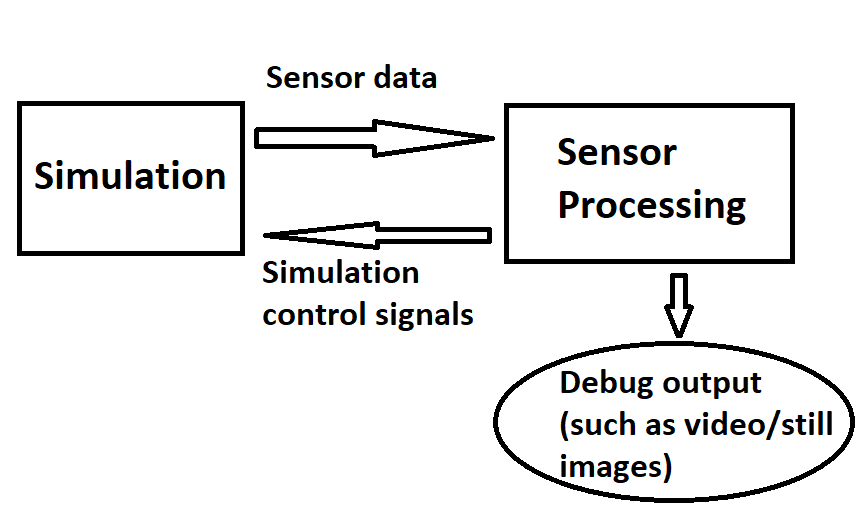
\includegraphics[width=0.5\textwidth, height=0.5\textwidth]{dataFlow.png}
	\caption{Anticipated data flow between simulation and sensor processing}
	\label{f:dataFlow}
\end{wrapfigure}

\subsection{Scope and Deliverables}\label{s:scope}

The scope of the project is deliberately kept constrained initially. This is to focus on the specific problem of localising a navigation route without losing development effort to supporting elements. As outlined previously the loose framing of this project is the goal of automating military field logistics route transport without tactical considerations. While the scope is initially narrowly defined it will be extended towards the end of the project as time and opportunity allow.

The scope and deliverables have been identified as follows:
\begin{easylist}[itemize]
	& The solution must be able to reconcile GPS and CV data to identify the current location and required direction to travel through intersections based on a navigation route.
	& \textbf{Limitation of road complexity.} There is a requirement for road/lane detection as part of this project (to marry up with the GPS polyline data) however optimised road detectioon is not the main focus of the project. Further as the project purely uses the output data of lane detection, it can be considered a `black box' and implementations can be swapped out as more advanced options are identified. The initial limitations on scope of road detection includes:
	&& Limit road detection to easily detectable road surface.
	&& Limit roads to single lane.
	&& All roads considered will be of similar local colour and type.
	& \textbf{Simulation deliverable requirements.} In addition to providing data for this project the intent is for the simulation to be held as an asset within SEIT for use in subsequent student projects in this area. The basic requirements for the simulation are:
	&& Ability to provide 3D video feed of simulated driving to external program.
	&& Support simulated GPS tracking data.
	&& Support simulation of GPS route guidance.
\end{easylist}

Based on the levels outlined in table \ref{t:automationLevels} the intended level is to level 2 or 3 for cognitive assistance and in automated remote logistics applications such as autonomously traversing known routes in a military field setting to facilitate the ability to control to level 4 autonomy.

\section{Project management}

Tracking of project progress is being maintained via a Gantt chart which is included as appendix \ref{app:ganttChart} and is updated at least fortnightly based on current work. In addition to this, the development of the simulation will use the Agile process with two week sprints with major monthly sprint reviews. Sprint tracking will be managed using Trello initially however may move to a more specialised solution as the project progresses.

\subsection{Project Methodology}

The initial state of the project was the field of autonomous vehicles as the general area of focus. As a result the preliminary phase of the project was the identification of the `problem area' and narrowing of scope. A broad reading of relevant research and industry articles identified the ability to navigate in arbitrary areas as a candidate problem area and the scope was refined as outlined in section \ref{sect:intro}. 

This project is being undertaken in an area of study that is a new field for the author. As a result the early focus was on developing base competencies in digital image processing and general computer vision. This included both an understanding of the theory and mathematics behind DIP and CV tools and familiarity with implementation options and extended into more specific areas such as straight lane detection.

In parallel with the CV competency development, research and experimentation on key technical risk elements of the simulation was conducted. The core technical risk was the ability for simulation code to communicate with sensor processing code. The aim was to keep these two code bases separate to allow other individuals to use the simulation for relevant purposes without being tied in to the aims of this project.

Once the core competencies have been developed and the supporting tool options have been analysed the focus will split between agile development of the simulation and the development of the external processing program. The simulation development will consist of `sprint' periods designed around providing incremental functionality, prioritised as needs arise. The development of the external processing forms the specific primary aim and will include the following core milestones:

\begin{easylist}[itemize]
	& Lane detection.
	& Intersection detection and identification of discrete roads.
	& Mapped road position estimation based off the GPS position and nearby road map nodes (accounting for GPS inaccuracy).
	& Map matching, specifically some form of curve or spline matching to correlate the estimated map position with the identified road features.
	& Consolidation of return data. This may include:
	&& Overlaying the navigation route directly to the video feed.
	&& Providing control inputs to the vehicle for autonomous driving of the route.
\end{easylist}

Additional considerations which will be addressed as part of the simulation development include the data structure representation of the GPS maps and navigation routes. These will both be in line with the OSM data structures but may be simplified to specifically the required data for ease of processing in testing. Simplification of data will only occur where it is feasible that the OSM (or similar) data format can be transformed into the used data format with sufficient preprocessing ie. only information that is present in, or able to be derived from, the OSM or similar data will be used.

\section{Current work}\label{s:currentWork}

The bulk of the initial effort has been developing technical competency within informing disciplines. This includes both the CV technical competency development and addressing the simulation technical risks. This completed work is tracked in the Gantt chart in appendix \ref{app:ganttChart}. Additionally to these aspects, familiarity projects were conducted on neural networks to consolidate the basic theory for potential future use. These projects consisted of developing neuroevolution based solutions for both a physics based ball balancing challenge over the duration of 5 minutes and custom cloned version of the mobile game `flappy bird'. Both solutions used a simple feedforward neural network coded in C\# without the use of any existing libraries with the networks evolving using a custom built genetic algorithm. The CV and simulation aspects are discussed in more detail in the following subsections. 

\subsection{Computer Vision}\label{s:currentWork_CV}

Before any effective computer vision approaches can be implemented a robust base of understanding of digital image processing is required. In order to develop a robust understanding of DIP concepts study was undertaken using a range of publicly available resources. The main resource used for structured learning was the Spring 2015 offering of ECSE-4540 at Rensselaer Polytechnic Institute in New York by Rich Radke which has the full set of recorded lectures freely available online. Basic algorithms were implemented from first principles in MATLAB which reinforced the internalisation of the concepts. More advanced computer vision concepts were subsequently researched and tested within Python using OpenCV functionality which is discussed further in this section. 

The Hough Transform was used to detect straight lanes with varying levels of success. The Hough Transform converts a global detection problem into a local peak detection problem in a parameter space \citep{surveyOfHT} where straight lines in an image can be represented by a single point in Hough space \citep{houghPaper}. A brief overview of simple lane detection, including a discussion on the Hough transform, is included as appendix \ref{app:briefOverviewOfLaneDetection}.

\begin{wrapfigure}{R}{0.5\textwidth} %this figure will be at the right
	\centering
	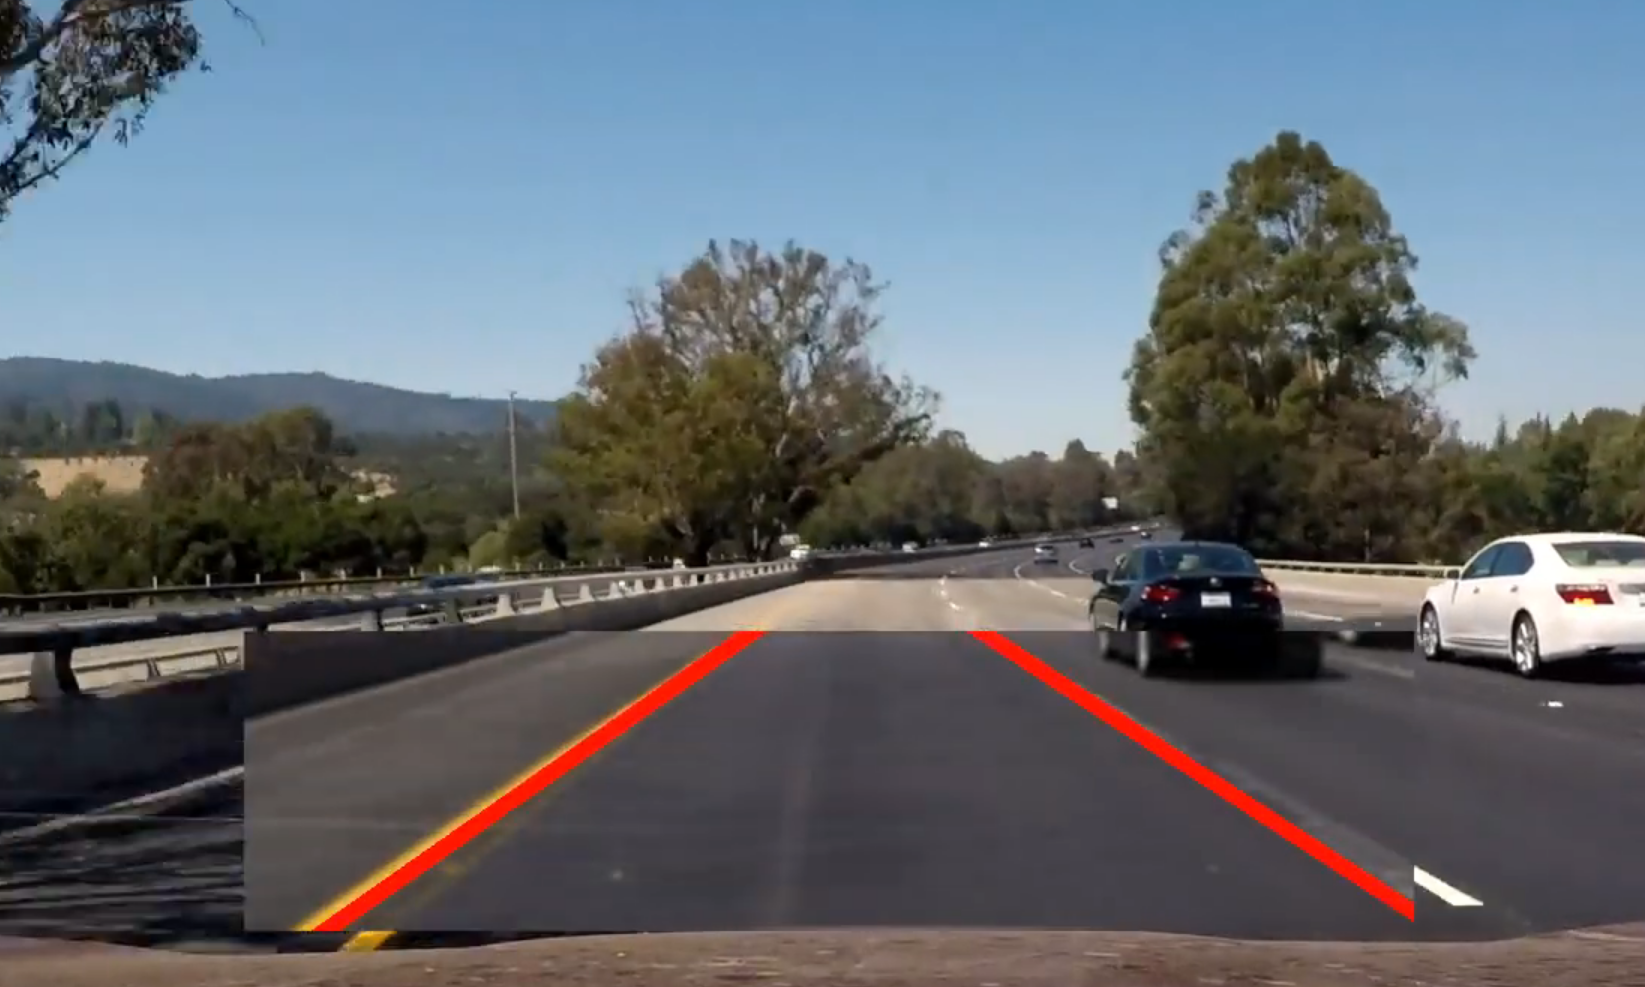
\includegraphics[width=0.5\textwidth, height=0.5\textwidth]{early_lane_detection_experiment.png}
	\caption{Still from video feed lane detection experiment. Lower area of interest where frames are averaged visible in the bottom central part of the image}
	\label{f:simpleLaneDetectionHough}
\end{wrapfigure}

It was noted that the simple approaches suffered when the dashed lane line was faint in comparison with other linear features and when the road was cast in intermittent shadow. The final experiment to improve on detection involved lane detection on a video feed using a rolling average of a lower area of interest of the most recent 5 frames of video as input to the lane detection for each frame. The lane detection approach involved identifying straight lines using the Hough Transform of the Canny edge detected area of interest after a low pass filter had been applied. The Hough lines were then chosen based on strength with the strongest line for each angle (side of the lane) chosen. The output consisted of the averaged area of interest with the detected lane lines in red overlayed onto the original frame. An example frame from the video output is included as figure \ref{f:simpleLaneDetectionHough}. 

In order to identify the true shape of the road, more advanced techniques are required. Inverse perspective mapping is `a geometrical transform that attempts to remove the perspective effect present in an image captured by a camera pitched down towards a road' \citep{intersectionDetectionSingleCamera}, allowing a birds eye view of the scene by weighing each pixel according to its information content \citep{stereoIPM}. Inverse perspective mapping has many uses within the autonomous driving realm including vanishing point detection  \citep{ipmVanishingPoint}, attitude noise reduction \citep{ipmAttitudeNoise}, distance determination \citep{ipmDistanceDetermination}, regularizing optical flow \citep{ipmOpticalFlow}, improving relative velocity determination \citep{ipmOpticalFlowSpeed} and detailed depth information in stereo \citep{stereoIPM}. Importantly though, inverse perspective mapping is a key part in effective lane and obstacle detection \citep{ipmOpticalFlow} \citep{ipmDistanceDetermination} \citep{ipmBasedLaneDetectionApproach} \citep{ipmVanishingPoint}.

The basic approach to lane detection using CV then involves correcting the image for camera lenses before inverse perspective mapping to get a `birds eye view' of the road. From this top down perspective, road/lane analysis can be conducted properly. An inverse perspective mapping calibration was developed using the interprocess communication implementation discussed in section \ref{s:currentWork}-\ref{s:simSystem}-\ref{s:IPC}. This calibration consists of still image of a checkerboard pattern on the horizontal plane within the simulation taken from the perspective of the camera. Corners of the checkerboard are manually identified in pixel space and the inverse perspective matrix is calculated based on the current old (perspective) and desired new (inverse perspective) positions. Automated identification of checkerboard corners is possible however the simulation camera rotation with reference to the horizontal plane is fixed therefore only a single calibration is required. The input and output of the inverse perspective mapping calibration undertaken is included as figure \ref{f:inverse_perspective_calibration}. Key considerations within the Computer Vision implementation decision process are in the following subsections.

\begin{figure}[htb]% order of placement preference: here, top, bottom
	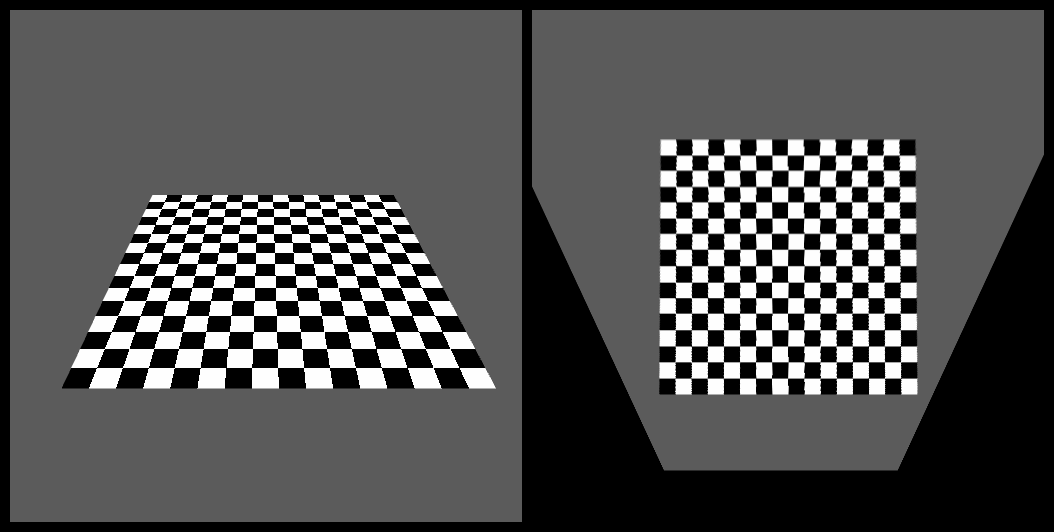
\includegraphics{InversePerspectiveEg.png}
	\caption{Inverse perspective mapping calibration. Original camera feed \textit{(left)} and inverse perspective mapped image \textit{(right)}}
	\label{f:inverse_perspective_calibration}
\end{figure}

\subsubsection{Use of OpenCV}\label{s:openCV}

The DIP theory that was undertaken opened up the possibility to implement the CV functionality from first principles, indeed basic tools such as filtering had already been implemented in MATLAB experiments. The alternative option considered was to use an open source computer vision library called OpenCV. OpenCV has C++, Python, Java and MATLAB interfaces and is widely used in commercial applications in companies such as Google, IBM and Honda \citep{opencvWebsite}. While implementing all functions manually has merit for further reinforcement of the basic principles, the decision was made to use the OpenCV library. Rationale for this includes the following: 

\begin{easylist}[itemize]
	& Efficient high performance vectorised implementations of CV algorithms.
	& Allows a greater proportion of time to be spent on solving the problem as opposed to implementing known algorithms.
	& Increase familiarity with industry level tools for future use.
\end{easylist}

\subsubsection{Language choice} \label{s:pythonVc}

Given the choice of OpenCV for the CV framework the options considered for the core language were C++ or Python. C++ has the advantage of being `lower level' however the OpenCV Python interface compiles down to the same C++ code so the only performance gains would be in the general program code as opposed to the CV implementations. Simulation engine considerations also played a part, as discussed in section \ref{s:currentWork}-\ref{s:simSystem}-\ref{s:simEngineChoice}, Unreal Engine uses C++ which would allow simulation code to talk directly to the OpenCV interface.

Despite the above advantages, C++ comes with an increased complexity and any speed gains require a robust understanding (and implementation) of memory management. By contrast, Python presents a lower barrier to entry while maintaining the OpenCV C++ vectorised optimisation. In addition, libraries such as numpy within Python present additional highly optimised operations for array data manipulation. The decision to use Unity for the simulation engine as discussed in section \ref{s:currentWork}-\ref{s:simSystem}-\ref{s:simEngineChoice} removed the major benefit of C++ simulation code being able to talk directly to OpenCV thus Python was determined to be the preferred language.

\subsection{Simulation system}\label{s:simSystem}

A significant element of the project deliverable is the development of the simulation system to provide sensor outputs. The intent of the simulation is to provide a pipeline of sensor feeds and potentially an interface to control a simulated vehicle based off the processed sensor data. The scope of the simulation is discussed in section \ref{sect:intro}-\ref{s:scope}. Key elements of the simulation system are discussed in the following subsections.


\subsubsection{Simulation engine} \label{s:simEngineChoice}

Two courses of action were available for the implementation of the simulation engine; development of a full custom simulation engine or implement within an existing game engine. For the existing game engine option, Unreal and Unity were both considered. A full custom engine allows fine grain control over the implementation the specific requirements of the simulation however has significant overheads including the implementation of 3D visuals including rendering, texturing and importing of 3D models. It was determined that this represented a very large time commitment for negligible benefit.

Both Unity and Unreal are professional 3D engines used in commercial games and computer graphics applications. They are well established and have a robust set of supporting tools. Specific considerations for each engine are as follows:

\begin{easylist}[itemize]
	& Unity:
	&& Personal experience with workflow and language (C\#). Comfortable implementing desired features.
	&& No C\# interface with OpenCV therefore interprocess communication will need to be developed between the OpenCV processing implementation and the simulation engine.
	& Unreal:
	&& New, unfamiliar workflow.
	&& Lack of familiarity and comfort with C++ which is used for scripting within the engine. `Blueprint' system does allow a visual programming approach although that represents an additional competency to be developed.
	&& C++ code allows direct interface with OpenCV.
\end{easylist}

When considering the above factors and the OpenCV considerations discussed in section \ref{s:currentWork}-\ref{s:currentWork_CV}-\ref{s:openCV}, Unity was chosen due to the ability to `hit the ground running' based on workflow and language familiarity. It was noted that this accepts a large technical risk of IPC implementation however it was deemed to be the preferred option.

\subsubsection{Interprocess Communication (IPC)} \label{s:IPC}

One of the main issues identified with using Python Open CV and the Unity game engine is the ability for simulation data, for example video feeds, to be transferred from Unity to the Python process. This was assessed as a significant technical challenge and is the single largest time budgeted feature in the initial simulation work. The motivation for fast IPC was to allow real time processing of the simulation data in order to allow for potential control feedback to the simulation. Transferring image data represents a large amount of memory thus has a significant time complexity per simulation `tick'. 

The initial research approach involved investigating options such as static memory buffers, shared memory and memory mapped files which would allow direct memory access to data. These options added another level of complexity and it was determined that a lower technical risk solution was to use TCP via the ZeroMQ middleware. ZeroMQ is a communications interface with implementations for both C\# and Python and is well optimised for speed.

 The use of this approach potentially results in slower than real time simulation processing which was mitigated by dynamic simulation time dilation, discussed in section \ref{sect:timedilation}. This approach allows easy and reliable two way communication which is required for effective feedback between the processes. This solution also offers the ability to expand off a single local machine, for example a hosted simulation with remote processing. While this is well out of scope of this research it presents additional flexibility for future development.

Once the IPC approach was confirmed, the data handling pipeline between the Unity (C\#) and Python processes was developed. The final simulation output data structure for video feed is a flattened 3D byte array with four bytes for each $(x,y)$ pixel coordinate, representing the Red, Blue, Green and Alpha image colour channels. 

The Python process casts the byte stream as a byte array and reshapes the data to a 3D array. The fourth element of each colour value (the Alpha channel) is redundant and is removed. This results in a final data structure consisting of a 2D array of 3 element vectors of bytes which is the required data structure for OpenCV processing operations. 

\subsubsection{Simulation time dilation}\label{sect:timedilation}

There is a requirement to implement dynamic time scaling in the simuation order to maintain time synchronisation with the external process. The simulation will scale time based on the desired processing update rate and the real time that the IPC process and external data processing takes. This allows simulation complexity scaling without the danger of temporal desynchronisation between simulation and external processes.

The implementation of time dilation involved a simulation controller that runs the simulation for a set time based off the desired sensor processing rate. After this time has elapsed, sensor data is collated and sent to the external processing program via the IPC process outlined above and the simulation pauses. On completion of the data processing, the external program sends an acknowledgement in return which triggers the next simulation tick. This has been implemented and tested by sleeping the processing thread for several seconds each tick. The time dilation was also tested using an initial prototype of the simulation in the same manner as the colour calibration discussed previously. Two stills from the Python process output video showing the raw feed and the canny edges is included as figure \ref{f:simPrototypeIPCTest}.

\begin{figure}[htb]% order of placement preference: here, top, bottom
 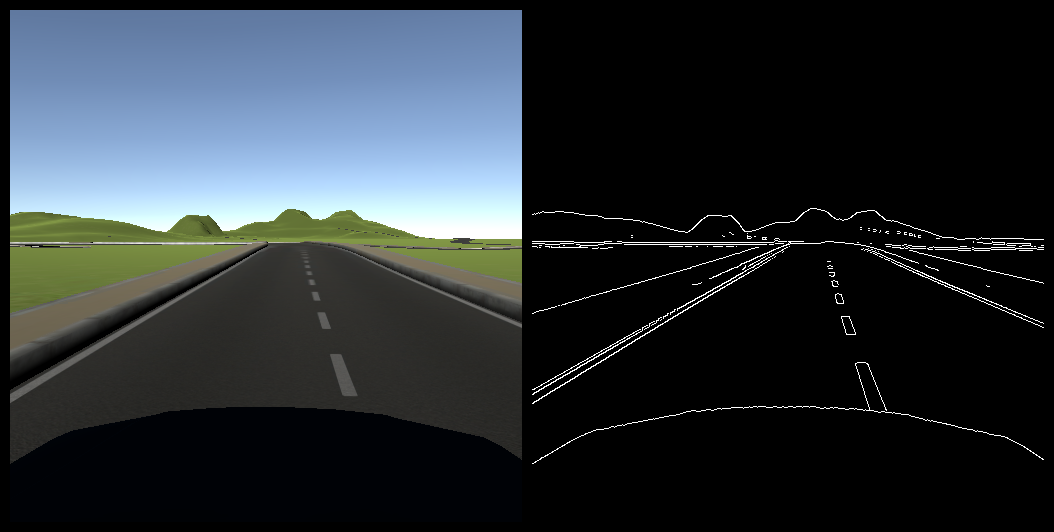
\includegraphics{simPrototypeIPC.png}
 \caption{Still from video feed of simulation prototype test. Original camera feed \textit{(left)} and canny edges of feed \textit{(right)}}
 \label{f:simPrototypeIPCTest}
\end{figure}

\section{Future work}

The work completed thus far has solved some key technical challenges required, in particular on the simulation side. The core areas of work in the remainder of the project, with the associated assessed technical risk, are discussed in the coming subsections. The Gannt chart included as appendix \ref{app:ganttChart} outlines the initial planned approach however this will be amended based on the realised complexity of each task.

\subsection{Computer Vision}

\subsubsection{Lane detection}

Detection of straight lane lines has been completed in the familiarisation activities conducted as discussed in section \ref{s:currentWork}-\ref{s:currentWork_CV} and demonstrated in figure \ref{f:simpleLaneDetectionHough}. Alternative approaches to lane detection which may be considered include k-means clustering \citep{ipmBasedLaneDetectionApproach} road classification from histogram based segmentation \citep{histogramSegmentationRoadClassification} road surface mapping from near field driving surface models \citep{darpaChallengeRoadDetection}, matching road curvature models to detected lane boundaries \citep{intersectionDetectionSingleCamera}  and open uniform B-spline model lane fitting \citep{ipmBasedLaneDetectionApproach}.

A more complex challenge is identifying a curved lane. Supervised convolutional neural network lane detection has had success through fully convolutional \citep{cnnLanes1} and instance segmented \citep{cnnLanes2} approaches. Spline based representation using random sample consensus for bezier splines based off road edge detection \citep{ransicBezierFit} has also shown to be effective. The current planned approach is lane edge detection via polynomial fitting of edge pixels detected by sliding window. An overview of the current implementation plan for the sliding window detection approach is included as appendix \ref{app:slidingWindow}. The technical risk of this aspect is low to medium.


\subsubsection{Intersection detection}

The SCARF (Supervised Classification Applied to Road Following) approach of using Gaussian colour models to identify road surface before road model matching \citep{scarf} and UNSCARF (UnSupervised Classification Applied to Road Following) approach using feature identification, clustering and edge detection and road model matching \citep{unscarf} have both demonstrated an ability to detect lanes and intersections in non ideal conditions using a dual camera setup, although not in real time \citep{scarfAndUnscarfPresented}. A data driven model using a `virtual camera' supported by model based intersection matching has also shown promise \citep{alvinnVC} however this requires prior information to reconstruct virtual images. Alternatively, once a binary road surface map is obtained, row based histograms can be used to identify intersection locations by interpolation between intersection models \citep{intersectionDetectionSingleCamera}.

Intersection detection presents a more challenging prospect than simple lane detection. The simplifying assumption of a single left and right lane edge is removed when intersections are introduced. One example of effective intersection detection as it applies to this project is model based recognition which matches intersection models to a series of road boundary points \citep{modelBasedIntersection}. An alternate approach is using skeletonisation of the road binary mask. When the full road surface is represented by a binary mask, skeletonisation will reduce each road to a single pixel line. This road skeleton can be matched to the model skeletons. The current intent is to use edge detection to determine boundary points with the intersection model being built reasonably simply using the OSM map data. The technical risk of this aspect is medium.


\subsection{Navigation localisation}

The final step involves correlating the GPS positional data, features from video sensor feed and the navigation data to localise the navigation data to the vehicle position. Static route map matching at its most trivial relates a GPS position to the nearest point on a polyline. It is anticipated that this will be the first step in the localisation to approximate the position on the navigation route. 

A LiDAR-based local trajectory generation has demonstrated through practical experiments that effective localisation using OSM data and global waypoints is possible using a LIDAR sensor suite \cite{mitLocalNavDriving}. General curve or spline matching options will be investigated and it has been identified that Markov and extended Kalman filter localisation techniques may also assist in this problem \citep{probabalisticRobotics}. The most likely solution will be a combination of the above and the model based recognition outlined by \citet{modelBasedIntersection}. The technical risk of this aspect is medium.

\subsection{Simulation}

The simulation development will follow the agile development process and deliver incremental feature additions and improvements. The basic features which are high priority for the early sprints are the implementation of the functionality required for the minimum viable product; the vehicle controller, the road network and the GPS sensor and navigation implementations. These aspects, as well as candidate functionality extensions are discussed in more detail in the coming subsections.

\subsubsection{Vehicle controller}

The vehicle controller will be implemented using the built in PhysX components within the Unity engine. The basic vehicle setup will consist of steering, accelerating and braking functions with vehicle movement simulated by the physics engine. An autopilot function that will follow defined waypoints from the navigation system discussed in section \ref{s:gpsNavSim} will also be developed. It is important to note that this autopilot is not based on the external analysis of sensor input but will use the exact game data. The intent of this functionality is to provide a constant video feed of a driving vehicle by a simulated driver agent for analysis and should not be confused with the autonomy solution to the main problem this research is investigating. Features such as engine power simulation will not be implemented in the initial stages but may be introduced as future features. The technical risk of this aspect is very low.

\subsubsection{Road network}

The road network is being implemented using a purchased tool called Easyroads 3D. This tool assists in mesh generation, placement, connection and texturing of roads as well as terrain moulding. Additionally the tool can accept map data exported from OSM. While each of these functions can be custom built individually it represents a significant time commitment and is unrelated to the core simulation. The road visible in the raw video feed of the IPC prototype test in figure \ref{f:simPrototypeIPCTest} demonstrates the implementation of a test road in Unity. The initial implementation of the road network will be simple single lane tracks. The technical risk of this aspect is low.

\subsubsection{GPS sensor}

The GPS sensor implementation is a simple function and required for the base sensor data analysis. The functionality will use the in engine coordinates for the GPS coordinates, as will all other data and sensors. An initial customisable random position offset will be used to simulate GPS positional error however additional functionality improvements may include a higher fidelity simulation of GPS error. The technical risk of this aspect is negligible.

\subsubsection{GPS navigation}\label{s:gpsNavSim}

The navigation functionality will initially be via hardcoded hand placed waypoints, using a simple queue system, with waypoint positions using the in engine coordinate system. Waypoints will be dequeued from a distance threshold based on GPS position proximity to the next waypoint. This represents the minimum viable product. There is significant room for expansion of functionality here including the ability to automatically route plan based off the OSM data used to build the road navigation network which can be queried using a path algorithm, most likely A*. This aspect has significant room for scope creep so will be managed tightly in the sprint reviews. The technical risk of this aspect is low to medium.

\subsubsection{Possible Extensions}

The implementation of further functionality is based on the sprint velocity achievable and the needs at the time. Once the minimum viable product with the above functionality is delivered it is likely that improvements to the existing functionality will take a high priority in future sprints however additional functionality will be considered in the sprint backlogs. Possible future extension ideas include:
\begin{easylist}[itemize]
	& External sensor definition files for automatic setup in simulation.
	& External OSM data file loading. Implementing this will also result in the requirement for automated data extraction from OSM files for simulated GPS and navigation rather than using hand placed nodes of interest.
	& Increased communication options between simulation and external process, for example vehicle control signals or specific sensor control/activation/deactivation.
	& 3D visual clutter such as trees.
\end{easylist}

\section{Conclusions}

The main technical risks for the sensor data processing include the detection of curved roads and intersections and the navigation localisation. Of these risks, the intersection detection is the most significant risk as it has the burden of providing an output that can be effectively used by the navigation localisation step. The main technical risks for the simulation have been successfully addressed and the development of the simulation is ready to enter the agile development process. This will deliver iterative improvements in functionality and provide a wealth of sensor data for analysis testing. Despite the identified risks, the research conducted has identified candidate solutions for each area of technical risk and rapid iteration through the areas of technical risk will assist in assessing the relative merit of the identified approaches.





%\section{Recommendations}
%This section should discuss and recommend directions for future work that will build on and extend your research and perhaps resolve some of the issues that you have encountered in your work.
%
%\section*{Acknowledgements}
%The Acknowledgements section should be used to briefly thank those individuals or organisations that have assisted you directly in your thesis work whether they be family, friends and colleagues, or technical and academic staff. Note that any external funding source that supported your project should be acknowledged here. 
%
\newpage
\section*{Appendices}
\ref{app:ganttChart} - Gantt chart \\

\ref{app:briefOverviewOfLaneDetection} - A brief overview of a simple approach to lane detection \\

\ref{app:slidingWindow} - Sliding window detection for curved roads \\

%Appendices may used to archive detailed summaries of data such as images, tables and charts and detailed example calculations such as for the estimation of measurement uncertainty. They may also include design drawings. Raw data, or detailed computer programs and files and extensive design drawings, should not be included. Their archiving should be discussed with your supervisor. Any appendices should be submitted as a SINGLE separate document file if referred to in the main text and be listed in the table of contents at the beginning (Note the use of a separate page numbering scheme).

% If you use MakeIndex
%\printindex


% AJL - UNCOMMENT THIS IS PREFERENCE TO THE ABOVE SECTION
%% produces the bibliography section when processed by BibTeX
\bibliography{InterimReferences}
%\bibliographystyle{aiaa}


\appendix
\pagestyle{empty}
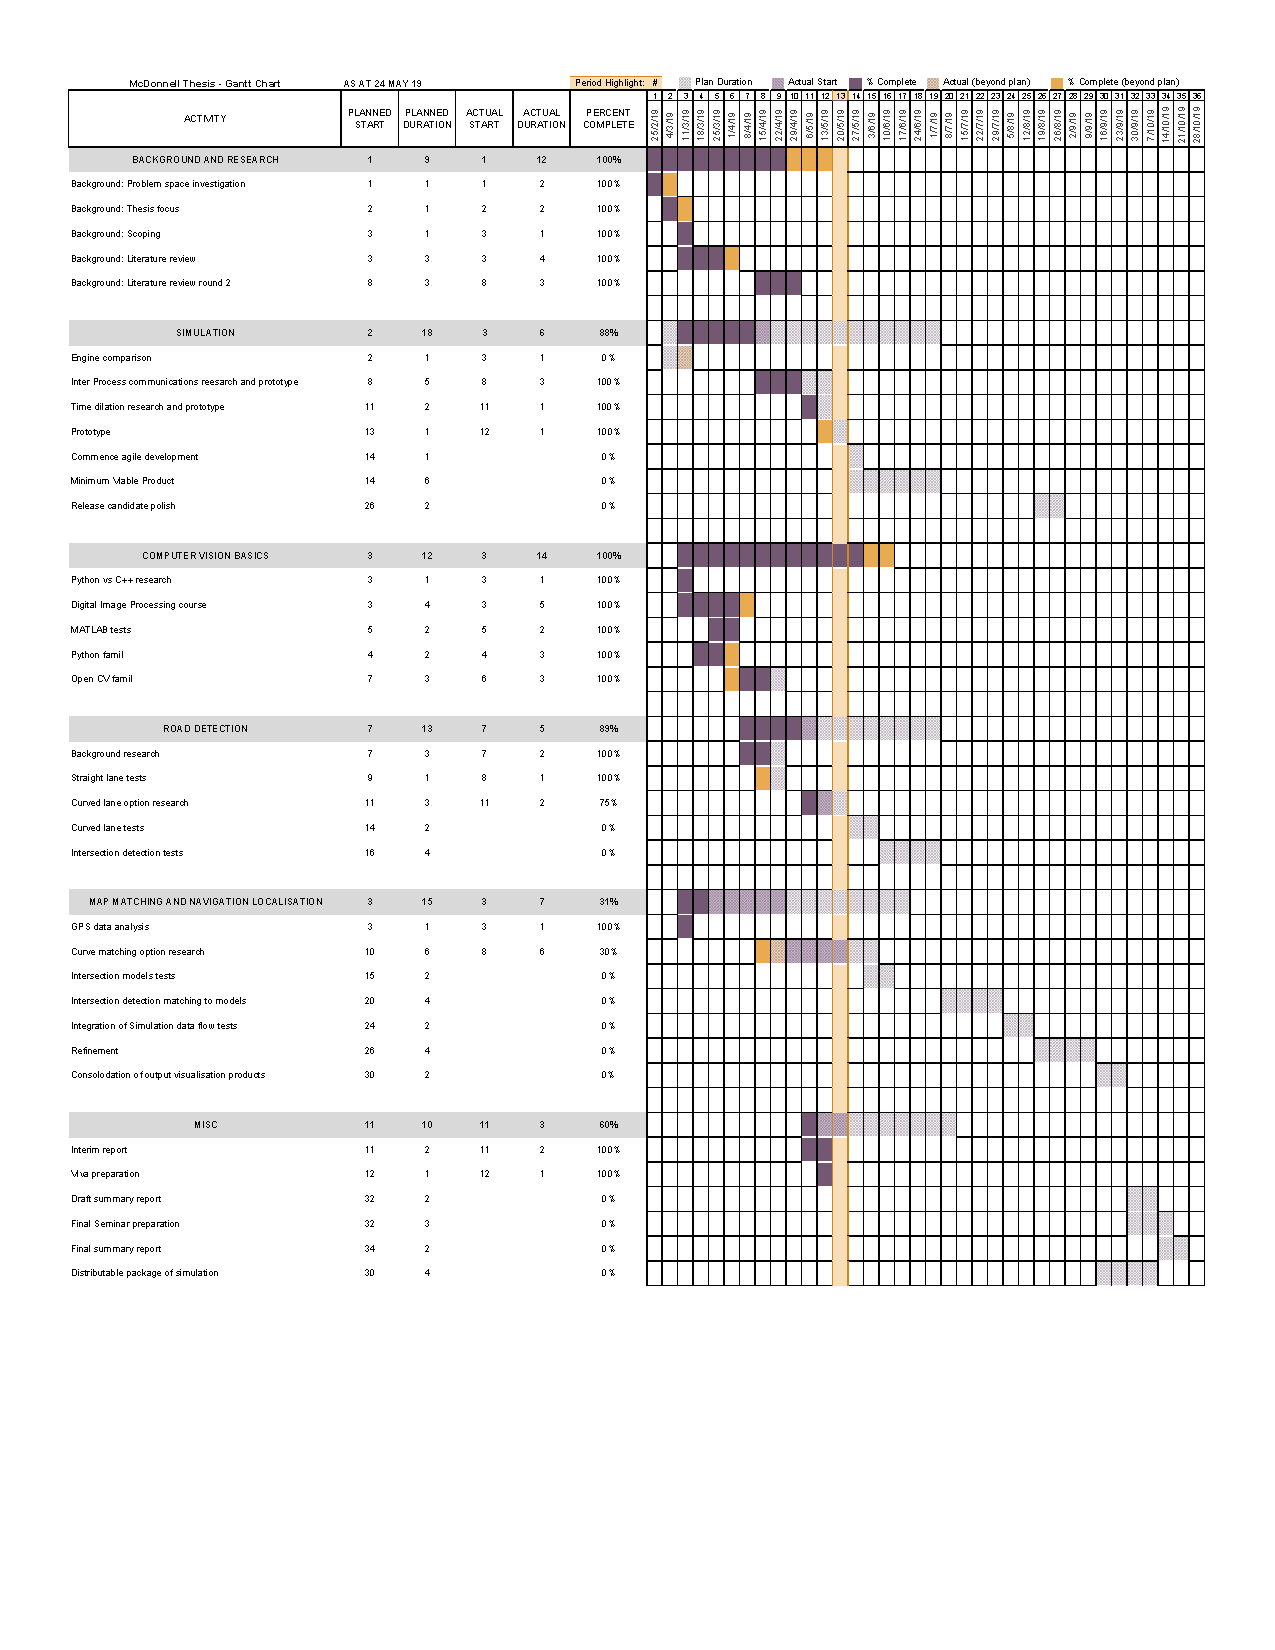
\includepdf[angle=-90,scale=0.9,pages=1,pagecommand=\section{Gantt Chart for Research Project}\label{app:ganttChart}]{GanttChart.pdf} 

%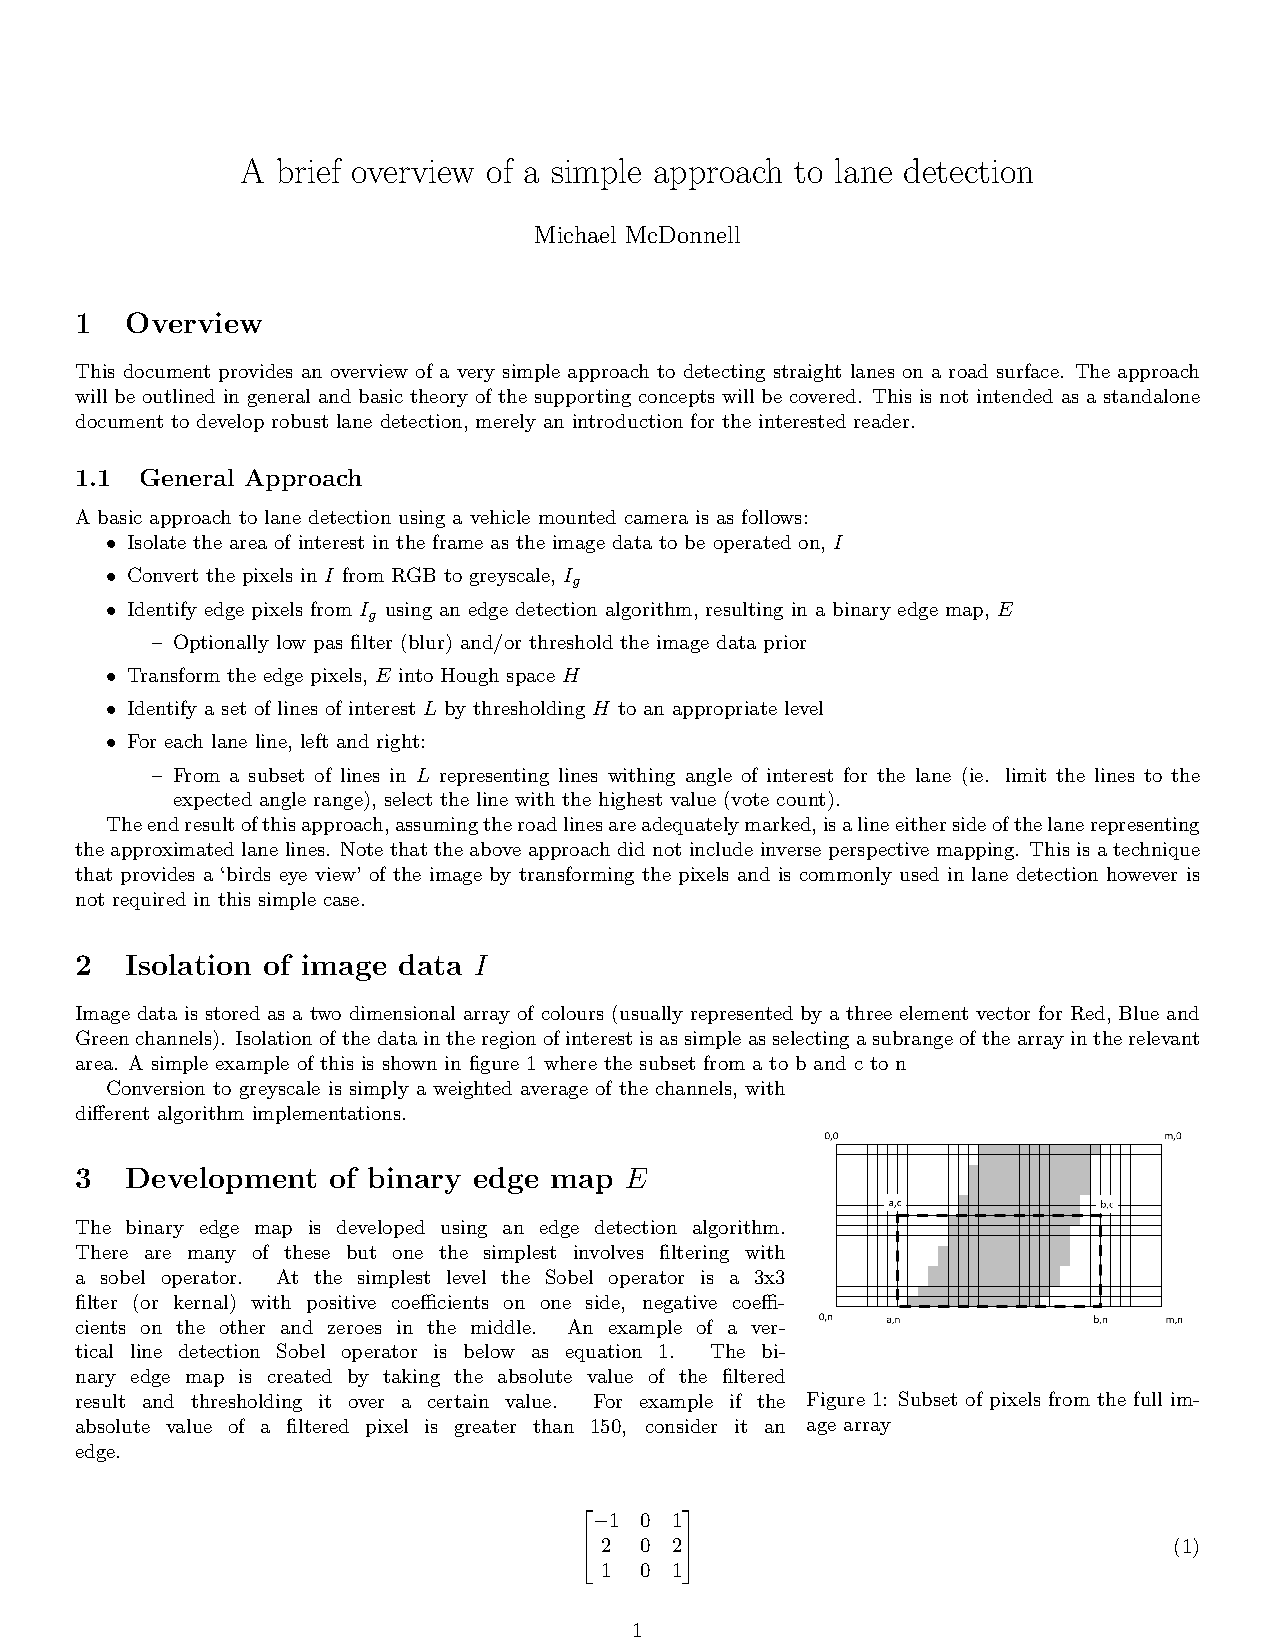
\includepdf[angle=0,scale=0.8,pages=1-,pagecommand=\section{A brief overview of a simple approach to lane detection}\label{app:briefOverviewOfLaneDetection}]{briefOverviewOfLaneDetection.pdf} 

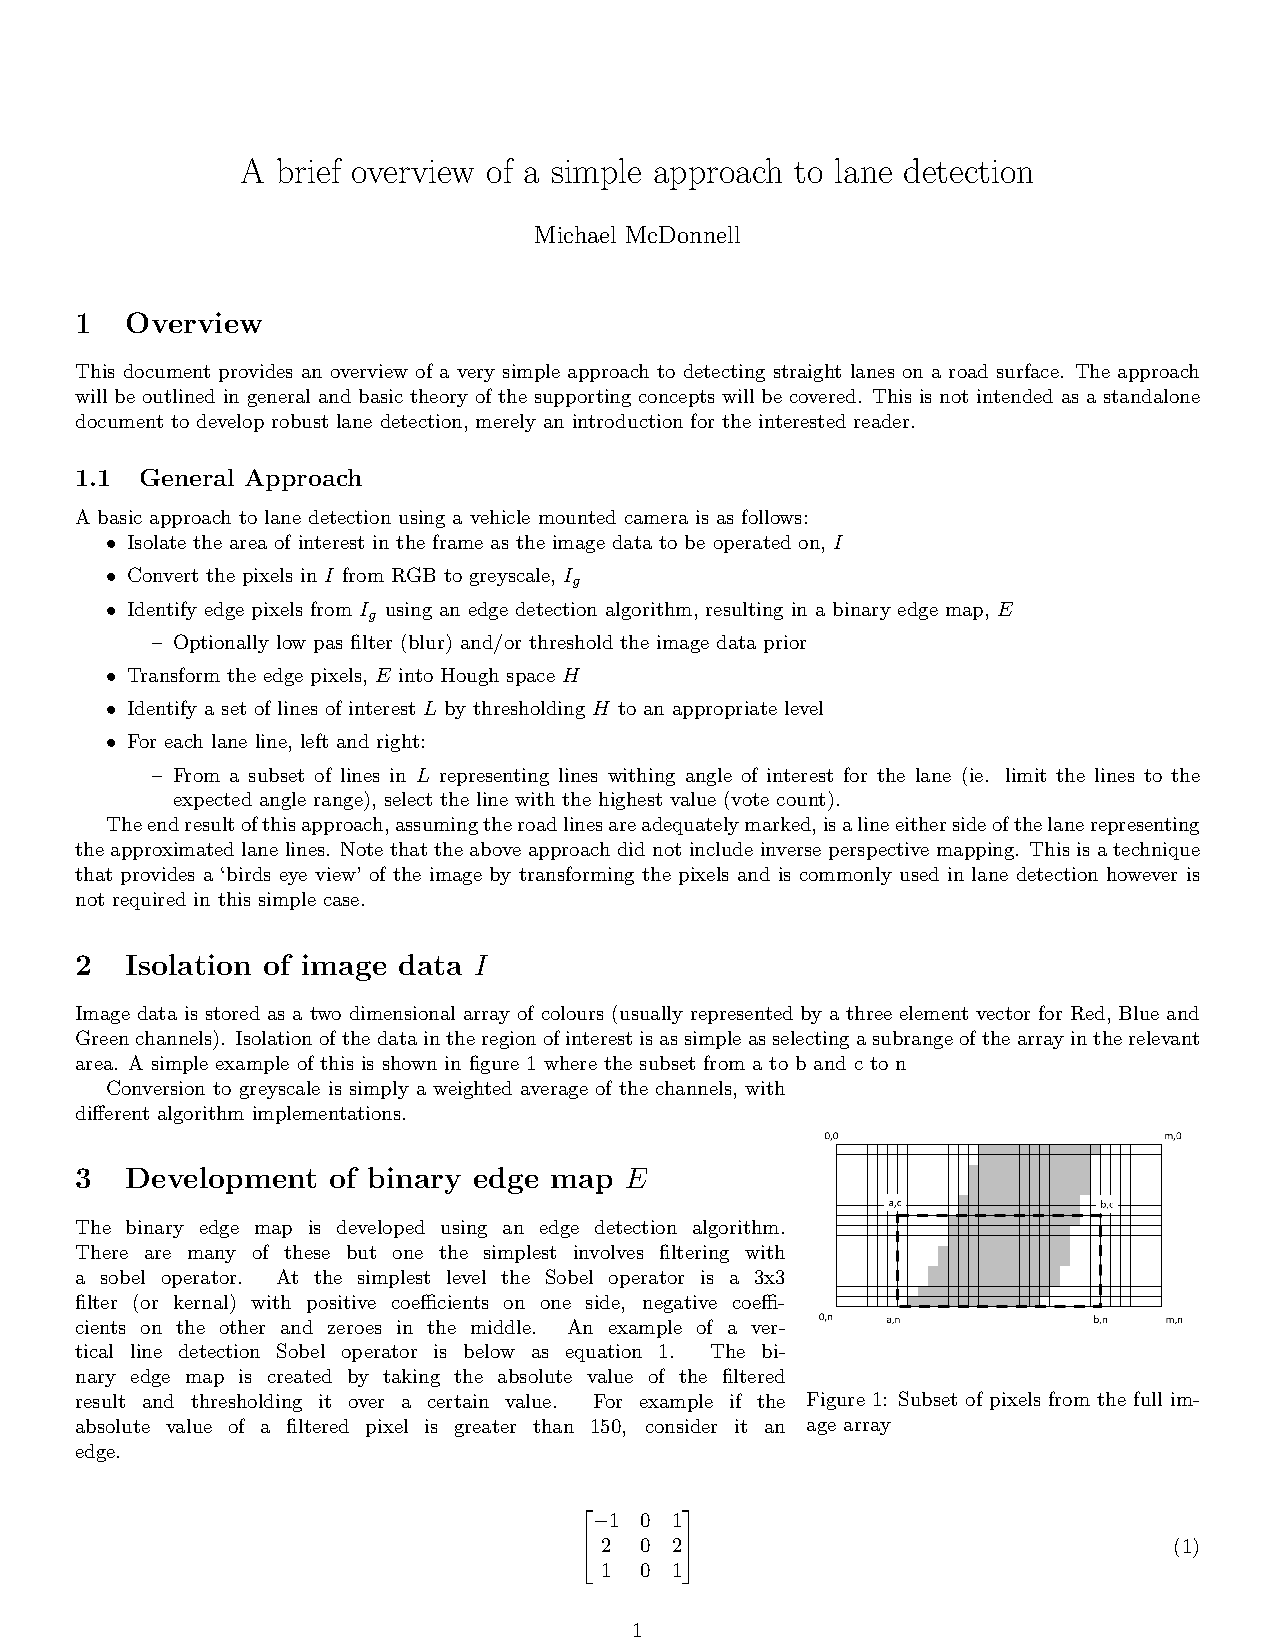
\includepdf[pages=1,scale=.8,pagecommand={\section{A brief overview of a simple approach to lane detection}\label{app:briefOverviewOfLaneDetection}},linktodoc=true]{briefOverviewOfLaneDetection.pdf}
\includepdf[pages=2-,scale=.8,pagecommand={},linktodoc=true]{briefOverviewOfLaneDetection.pdf}

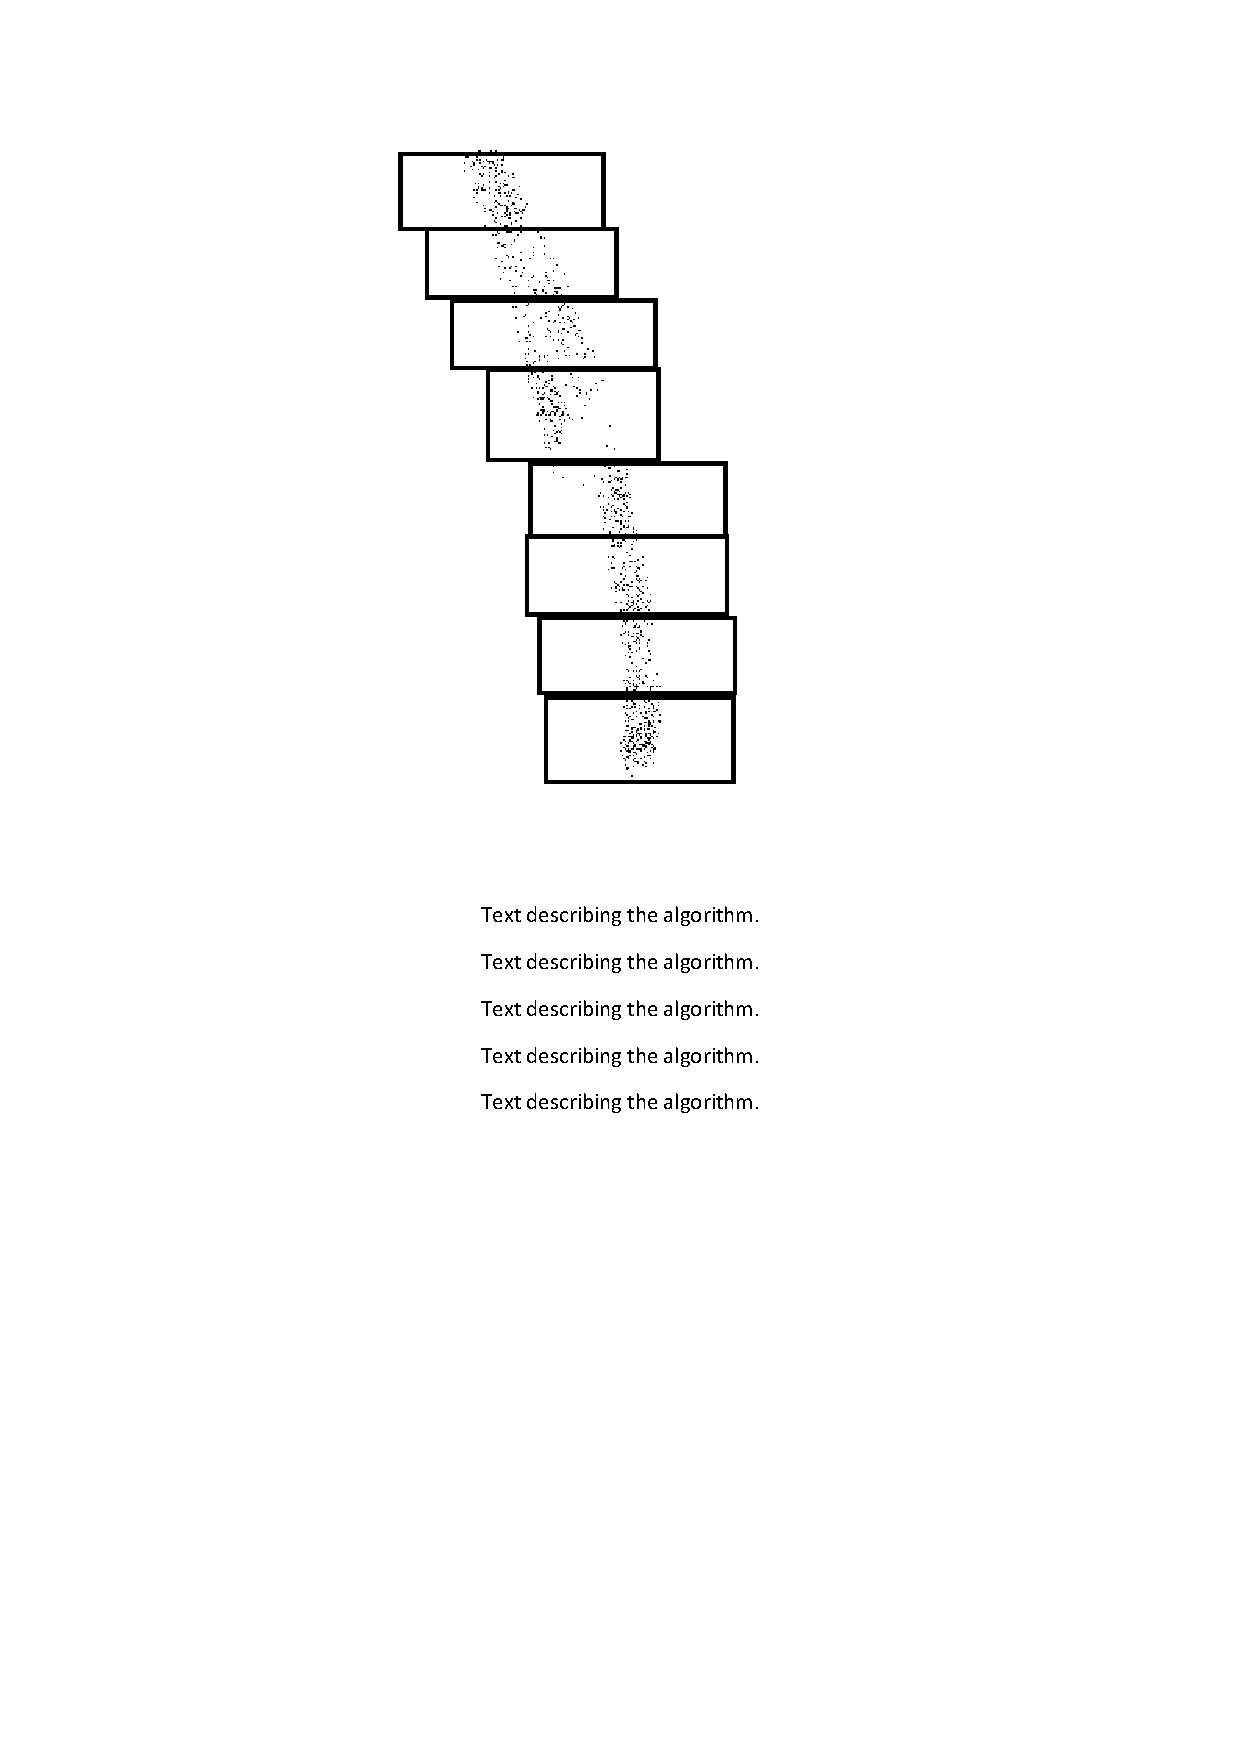
\includepdf[angle=-90,scale=0.9,pages=1,pagecommand=\section{Sliding window detection for curved roads}\label{app:slidingWindow}]{curvedLaneDetection.pdf} 

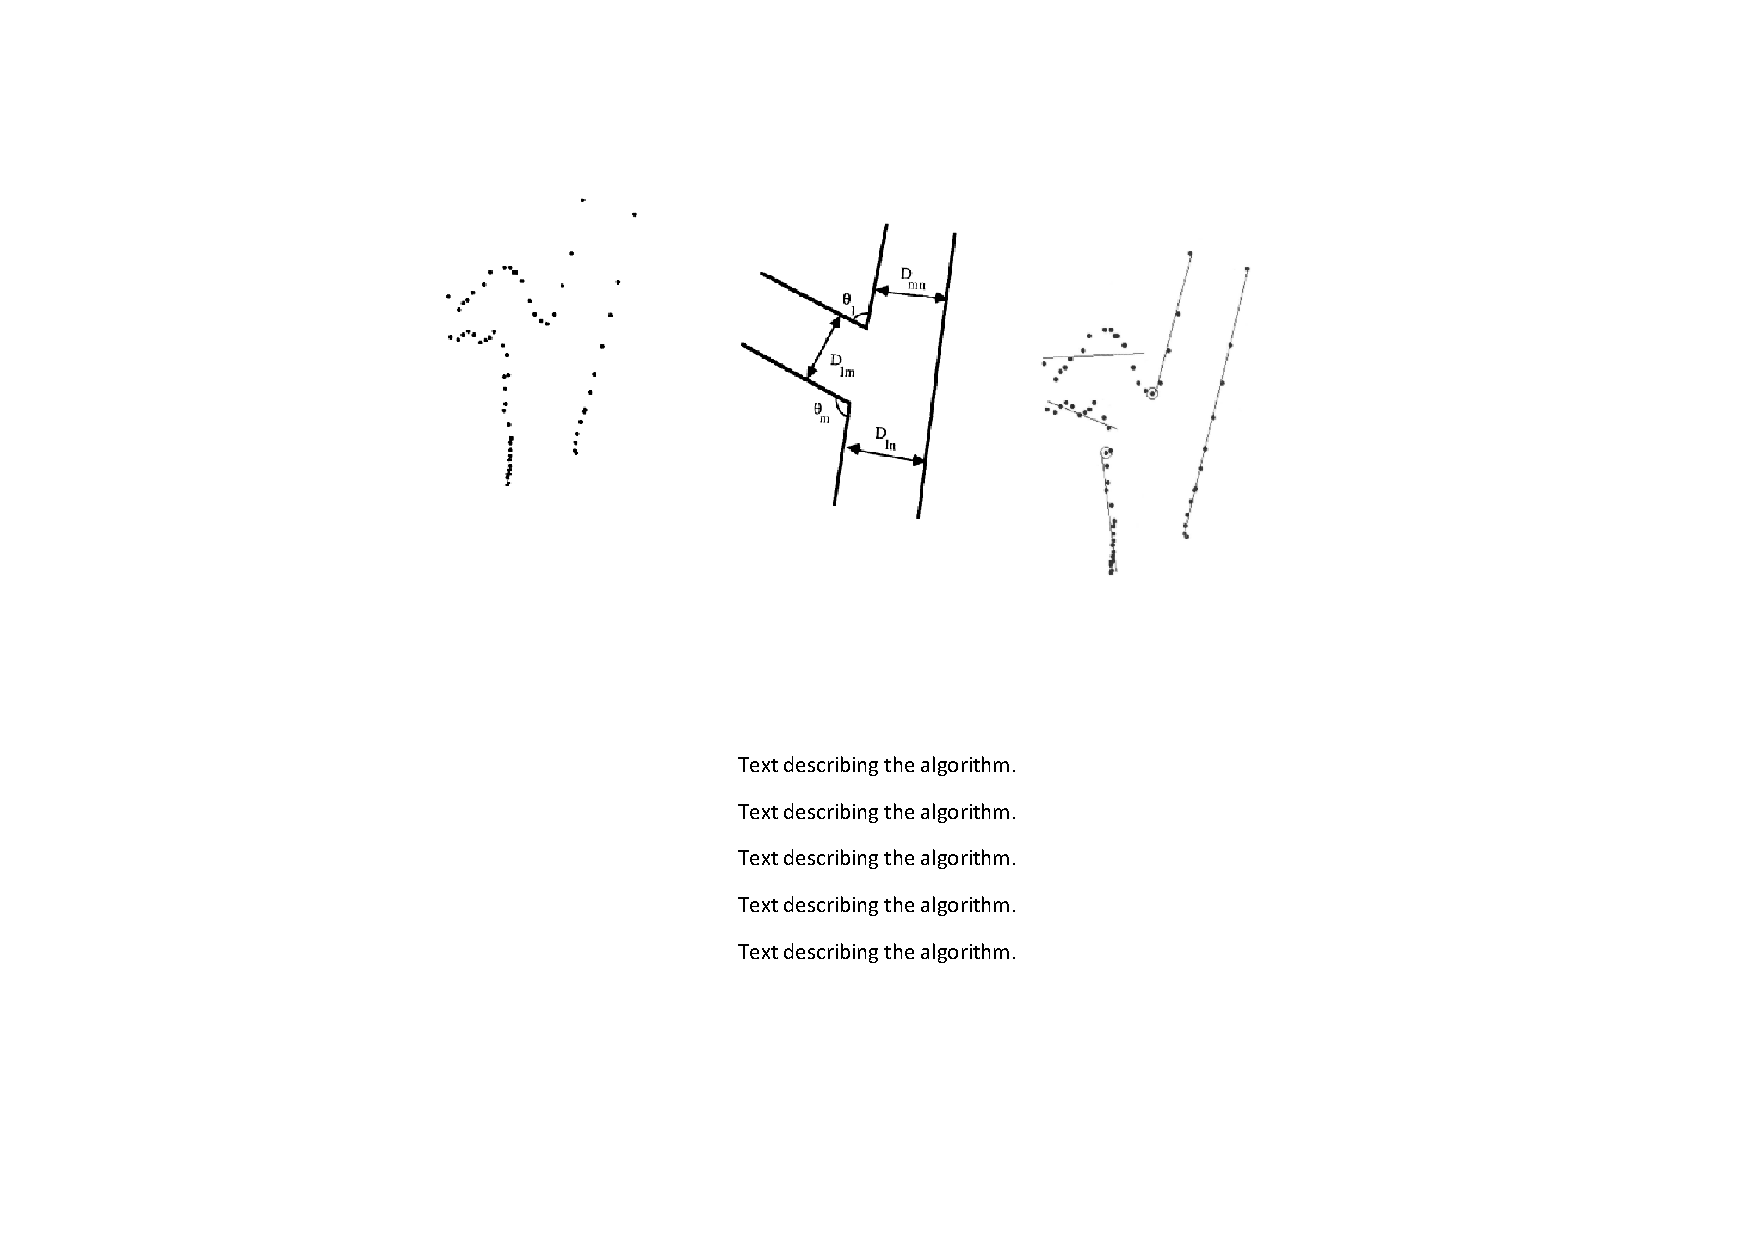
\includepdf[angle=-90,scale=0.9,pages=1,pagecommand=\section{Model based intersection detection approach}\label{app:modelDetection}]{modelBasedDetection.pdf} 


\end{document}

